\documentclass[oneside]{book}

\usepackage{graphicx}
\graphicspath{ {./images/} }
\usepackage{amsthm}

\theoremstyle{definition}
\newtheorem{definition}{Definition}[section]

\title{Dispensa Intro to Machine Learning}
\author{Bonmassar Ivan}

\begin{document}
	\maketitle
	\tableofcontents
	
\chapter{ML Basics}
The main notion to get from this is the following. ML allows computers to gain \textbf{knowledge} acquired through \textbf{algorithms} by learning from data. This knowledge is represented through a \textbf{model} which is then used on future data.

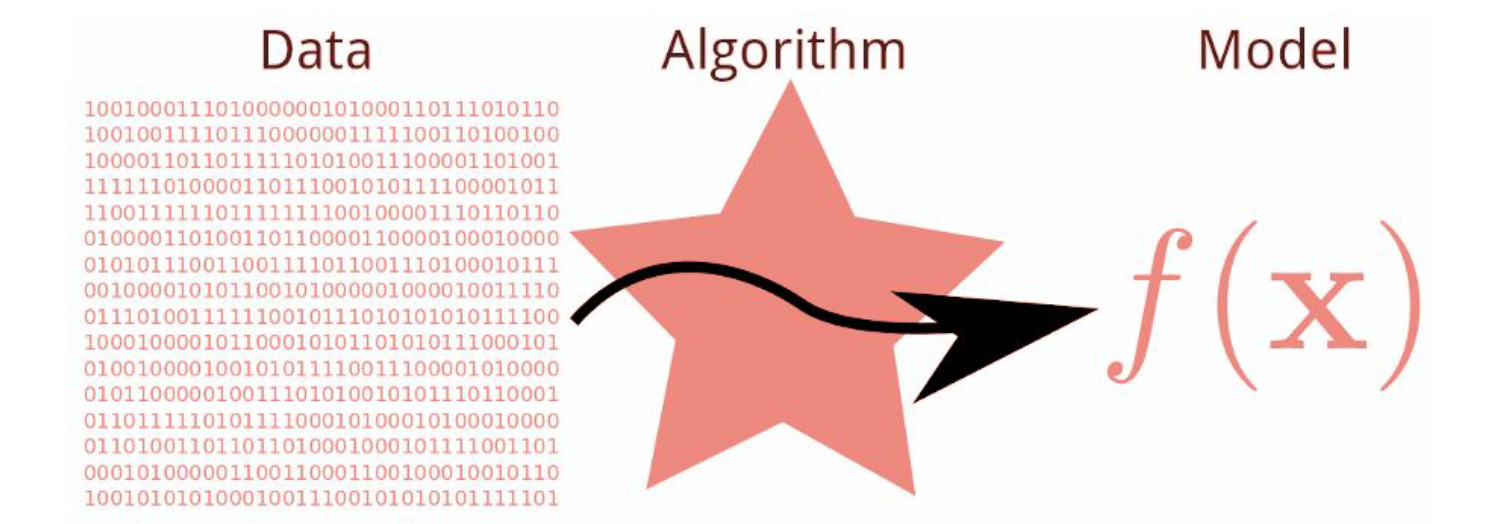
\includegraphics[scale=0.25]{data_model}

The training data produces a model or predictor, whereas the testing data produce a prediction. 
\section{Data}
Data can be a list of movies from IMDB which is easily representable. Although we need to use \textbf{features} when taking into consideration other examples. Features is how an algorithm view data and is generally represented with vectors. 

For example, classifying different apples, features could be the shape and colour of them.

The general problem with data for classification for example is that not all data is the same. For instance a banana can either be green or yellow. Although this is true we cannot go to deep with this so we use a probabilistic model called \textbf{data generating distribution}. Both training and test data are based on this. 

So in our previous example, we will generalize and say that bananas are yellow. 

\begin{definition}[Probability distribution]
	Describes how likely certain events are.
\end{definition}

\section{Types of Learning}
\textbf{SUPERVISED LEARNING}\\
Supervised learning is when the algorithm is given labeled examples and the predictor should output a label. A further example of this is \textbf{classification}, where the model classifies from a pool of categories. 

Given a training set $T = {(x_i, y_i)}$ learn a function that predicts $y$ given $x$. x is multi-dimensional.

Some real world examples can be facial recognition, spam detection and character recognition. 

\textbf{Regression} is similar to classification only with real values (i.e. numbers).

\textbf{Ranking} the label is a ranking (most similar, most popular web pages etc.)


\textbf{UNSUPERVISED LEARNING}
The given data is without labels. 
Some examples are: 

\textbf{Clustering}, where the output is the general structure of the data set (clusters of data). Real world examples are image segmentation, social network analysis 

\textbf{Anomaly detection}

\textbf{Dimensionality reduction} 

\textbf{REINFORCEMENT LEARNING}

The idea is that the agent interacts with the environment and receives rewards based on behavior. 




\end{document}